\documentclass[crop,tikz]{standalone}
\usetikzlibrary{%
    arrows,
    arrows.meta,
    automata,
    backgrounds,
    calc,
    decorations.pathreplacing,
    fit,
    matrix,
    positioning,
    scopes,
    shadows
}
\usepackage[linguistics]{forest}
\usepackage[charter]{mathdesign}
\tikzset{headarrow/.style = {-{Latex[length=.5em]}}}
\tikzset{dominance/.style = {dashed, blue, -{Latex[length=.5em]}}}

\begin{document}
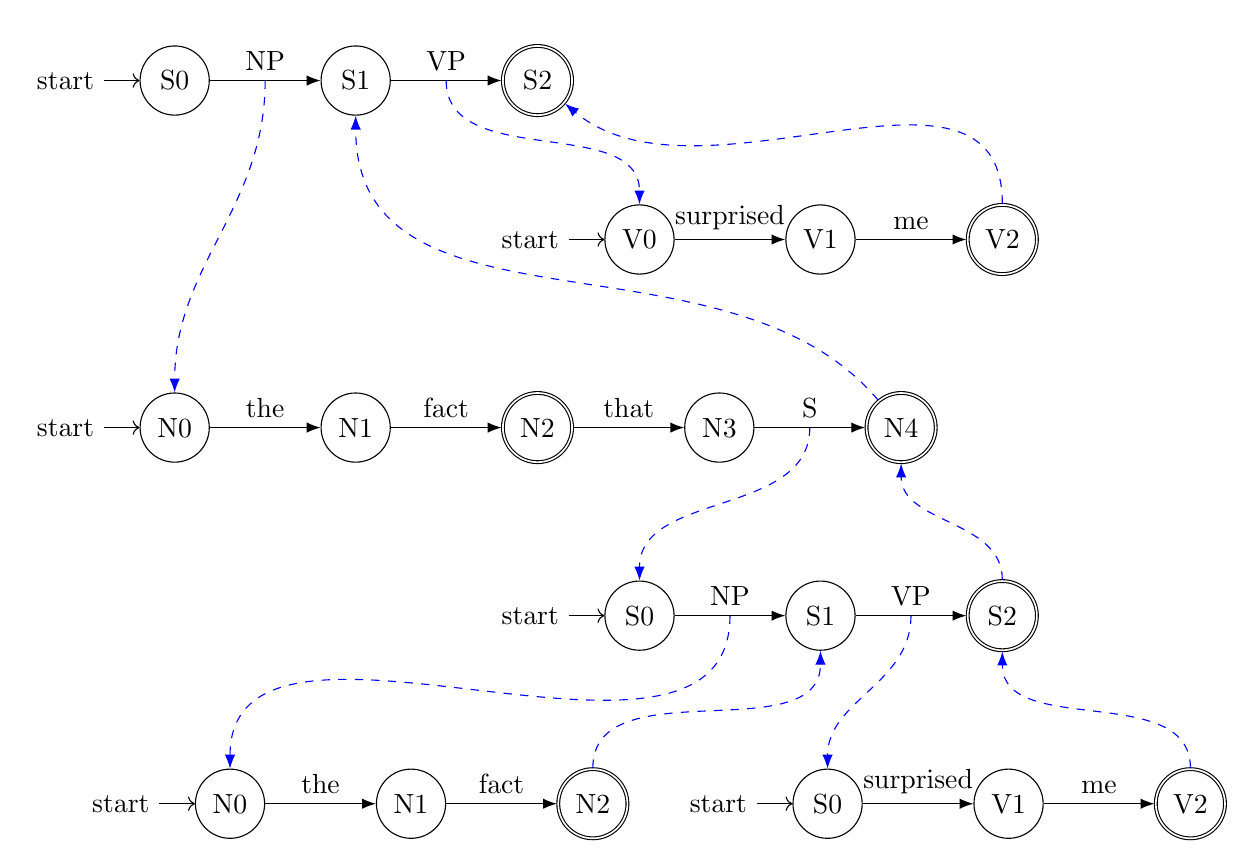
\begin{tikzpicture}
    % automata starts
    \node[state,initial] (S0) at (0,0) {S0};
    \node[state,initial] (N0) [below=10em of S0] {N0};
    \node[state,initial] (V0) [above right=5em and 15em of N0] {V0};
    \node[state,initial] (S'0) [below right=5em and 15em of N0] {S0};
    \node[state,initial] (N'0) [below left=5em and 13em of S'0] {N0};
    \node[state,initial] (V'0) [below right=5em and 5em of S'0] {S0};

    % other states
    \foreach \Aut in {S,N,V}
        {
        \node[state]           (\Aut1) [right=4em of \Aut0]  {\Aut1};
        \node[state,accepting] (\Aut2) [right=4em of \Aut1]  {\Aut2};
        }
    \foreach \Aut in {S,V,N}
        {
        \node[state]           (\Aut'1) [right=4em of \Aut'0]  {\Aut1};
        \node[state,accepting] (\Aut'2) [right=4em of \Aut'1]  {\Aut2};
        }

    % add center embedding
    \node[state] (N3) [right=4em of N2] {N3};
    \node[state,accepting] (N4) [right=4em of N3] {N4};

    % edges
    \foreach \Source/\Target/\Label in {%
        S0/S1/NP,
        S1/S2/VP,
        S'0/S'1/NP,
        S'1/S'2/VP,
        N0/N1/the,
        N1/N2/fact,
        N'0/N'1/the,
        N'1/N'2/fact,
        N2/N3/that,
        N3/N4/S,
        V0/V1/surprised,
        V1/V2/me,
        V'0/V'1/surprised,
        V'1/V'2/me%
        }
        \draw[headarrow] (\Source) to node (\Source-label) [above] {\Label} (\Target);

    % connections between automata
    \foreach \Source/\Target in {%
        S0/N0,
        S1/V0,
        N3/S'0,
        S'0/N'0,
        S'1/V'0%
        }
        \draw[dominance, out=270, in=90] (\Source-label) to (\Target);
    \foreach \Source/\Target in {%
        S'2/N4,
        N'2/S'1,
        V'2/S'2%
        }
        \draw[dominance, out=90, in=270] (\Source) to (\Target);
    \draw[dominance, out=130, in=270] (N4) to (S1);
    \draw[dominance, out=90, in=320] (V2) to (S2);
\end{tikzpicture}
\end{document}
